%% Appendix

\section{From names to de Bruijn indices and back}
\label{from_to_deBruijn}

The syntax of the \picalc{} \cite{Sangio01} using channel names is given by the $\Raw$ grammar below:
\begin{mathpar}
  \datatype
  { }
  {\Raw : \Set}
  \; \textsc{Raw}
\end{mathpar}

\begin{equation*}
  \begin{aligned}
    \Raw ::= &\; \PO              &&\text{(inaction)}    \\ 
    |& \; (\new{\Name}) \; \Raw         &&\text{(restriction)} \\ 
    |& \; \comp{\Raw}{\Raw}       &&\text{(parallel)}    \\ 
    |& \; \recv{\Name}{\Name}\Raw &&\text{(input)}       \\ 
    |& \; \send{\Name}{\Name}\Raw &&\text{(output)}      \\
  \end{aligned}
\end{equation*}

Channel names and variables range over $x,y,z$ in $\Name$ and processes over $P,Q,R$ in $\Raw$.
Process $\PO$ denotes the terminated process, where no further communications can occur.
Process $(\new{}x)\; P$ creates a new channel $x$ bound with scope $P$.
Process $\comp{P}{Q}$ is the parallel composition of processes $P$ and $Q$.
Processes $\recv{x}{y} P$ and $\send{x}{y} P$ denote respectively, the input and output processes of a variable $y$ over a channel $x$, with continuation $P$.
Scope restriction $(\new{}x) \; P$ and input $\recv{x}{y} \; P$ are \emph{binders}, they are the only constructs that introduce bound names --- $x$ and $y$ in $P$, respectively.

In order to demonstrate the correspondence between a \picalc{} that uses names and one that uses de Bruijn indices, we provide conversion functions in both directions and prove that they are inverses of each other up to $\alpha$-conversion.

\paragraph*{From names to de Bruijn indices}
When we translate into de Bruijn indices we keep the original binder names around --- they will serve as name hints for when we translate back.
The translation function $\func{fromRaw}$ works recursively, keeping a context $ctx : \Names_n$ that maps the first $n$ indices to their names.
Named references within the process are substituted with their corresponding de Bruijn index.
We demand that the original process is well-scoped: that all its free variable names appear in $ctx$ --- this is decidable and we therefore automate the construction of such a proof term.
\begin{alignat*}{2}
    &\func{fromRaw} && : (ctx : \Names_n) \; (P : \Raw) \\
    &               && \to \WellScoped \; ctx \; P \to \Process_n
\end{alignat*}

\paragraph*{From de Bruijn indices to names}
The translation function $\func{toRaw}$ works recursively, keeping a context $ctx : \Names_n$ that maps the first $n$ indices to their names.
As some widely-used languages do, this translation function produces unique variable names.
These unique variable names use the naming scheme $<namehint>^{<n>}$, where $^{<n>}$ denotes that the name $<namehint>$ has already been bound $n$ times before.
\begin{equation*}
    \func{toRaw} : (ctx : \Names_n) \to \Process_n \to \Raw
\end{equation*}

\begin{example}[$\func{fromRaw}$ and $\func{toRaw}$]
  We illustrate the conversion functions from names to de Bruijn indices $(\func{fromRaw}$) and back ($\func{toRaw}$) with three processes $P,Q,R$  below.
  \begin{alignat*}{7}
    &P = (\new{x} ) && (\comp {\recv{x}{x} && \send{x}{z} && \PO} {(\new{y}) && (\send{x}{y} && \recv{y}{y} && \PO)}) \\
    &Q = \new{} && (\comp {\recv{0}{} && \send{0}{2} && \PO} {\new{} && (\send{1}{0} && \recv{0}{} && \PO)}) \\
    &R = (\new{x^0} ) && (\comp {\recv{x^0}{x^1} && \send{x^1}{z^0} && \PO} {(\new{y^0}) && (\send{x^0}{y^0} && \recv{y^0}{y^1} && \PO)})
  \end{alignat*}

  Process $P$ uses names $x,y,z$ and is translated via the conversion function $\func{fromRaw}$ into process $Q$, which uses de Bruijn indices.
  Process $Q$ is then translated via $\func{toRaw}$ into process $R$, which follows the \emph{Barendregt convention}\footnote{The Barendregt variable convention states that all bound variables/names in a process are distinct among each other and from the free variables/names.} and is $\alpha$-equivalent to the original process $P$.
\end{example}

In the following we present the main results that our conversion functions satisfy.

\begin{nilemma}
  Translating from de Bruijn indices to names via $\func{toRaw}$ results in a well-scoped process.
\end{nilemma}

\begin{nilemma}
  Translating from de Bruijn indices to names via $\func{toRaw}$ results in a process that follows the \emph{Barendregt convention}.
\end{nilemma}

\begin{nilemma}
  Translating from de Bruijn indices to names and back via $\func{fromRaw} \circ \func{toRaw}$ results in the same process modulo internal variable name hints.
\end{nilemma}

\begin{nilemma}
  Translating from names to de Bruijn indices and back via $\func{toRaw} \circ \func{fromRaw}$ results in the same process modulo $\alpha$-conversion.
\end{nilemma}

\begin{proof}
  All the above results are proved by induction on \textsc{Process}, \textsc{Var} (\autoref{def:syntax}) and \textsc{Raw}.
  Complete details can be found in our mechanisation in Agda in \cite{Zalakain2020Agda}.
\end{proof}

%%%%%%%%%%%%%%%%%%%%%%%%%%%%%%%%%%%%%%%%%%%%%%%%%%%%%%%%%%%%%%%%%%%
\section{Type Safety} \label{app:type-safety}

\paragraph*{Exchange}
This property states that the exchange of two variables preserves the well-typedness of a process.
We extend $\func{exchange}_i$  introduced in \autoref{def:equals} to exchange types in typing contexts and usage annotations in usage contexts.
\begin{nitheorem}[Exchange]
  \label{thm:exchange}
  Let $P$ be well typed in $\types{\gamma}{\Gamma}{P}{\Xi}$.
  Then, $\types{\func{exchange}_i \; \gamma}{\func{exchange}_i \; \Gamma}{\allowbreak \func{exchange}_i \; P}{\func{exchange}_i \; \Xi}$.
\end{nitheorem}

\begin{proof}
  All the above theorems are proved by induction on \textsc{Types} and \textsc{VarRef}.
  For details, refer to our mechanisation in Agda \cite{Zalakain2020Agda}.
\end{proof}

\paragraph*{Subject Congruence}
This property states that applying structural congruence (\autoref{def:equals}) to a well-typed process preserves its well-typedness.
To prove this result, we must first introduce lemmas that establish that certain syntactic manipulations can be inverted (\autoref{lm:lower-lift}, \autoref{lm:exchange-exchange}) and how unused variables relate to the preservation of leftovers (\autoref{lm:types-unused}).

\begin{nilemma}
  \label{lm:lower-lift}
  The function $\func{lower}_i \; P \; uP$ has an inverse $\func{lift}_i \; P$ that increments every $\textsc{Var}$ greater than or equal to $i$, such that $\func{lift}_i \; (\func{lower}_i \; P \; uP) \equiv P$.
\end{nilemma}
\begin{proof}
  By structural induction on \textsc{Process} and \textsc{Var}.
\end{proof}

\begin{nilemma}
  \label{lm:exchange-exchange}
  The function $\func{exchange}_i \; P$ is its own inverse: $\func{exchange}_i \; (\func{exchange}_i \; P) \equiv P$.
\end{nilemma}
\begin{proof}
  By structural induction on \textsc{Process} and \textsc{Var}.
\end{proof}

\begin{nilemma}
  \label{lm:types-unused}
  For all well-typed processes $\types{\gamma}{\Gamma}{P}{\Xi}$, if the variable $i$ is unused within $P$, then $\Gamma$ at $i$ is equal to $\Xi$ at $i$.
\end{nilemma}
\begin{proof}
  By induction on \textsc{Process} and \textsc{Var}.
\end{proof}

We are now in a position to prove subject congruence.

\begin{nitheorem}[Subject congruence]
  \label{thm:subject-congruence1}
  If $P \eq{} Q$ and $\types{\gamma}{\Gamma}{P}{\Xi}$, then $\types{\gamma}{\Gamma}{Q}{\Xi}$.
\end{nitheorem}

\begin{proof}
  The proof is by induction on \textsc{Equals} $\eq{}$.
  Here we only consider those cases that are not purely inductive: the base cases for $\constr{struct}$ and their symmetric variants.
  Full proof in \cite{Zalakain2020Agda}.
  We proceed by induction on \textsc{StructCong} $\eqeq$:
  \begin{itemize}
    \item
      Case $\constr{comp-assoc}$: trivial, as leftover typing is naturally associative.
    \item
      Case $\constr{comp-sym}$ for $\comp{P}{Q}$: we use framing (\autoref{thm:framing}) to shift the output context of $P$ to the one of $Q$; and the input context of $Q$ to the one of $P$.
    \item
      Case $\constr{comp-end}$: trivial, as the typing rule for $\PO$ has the same input and output contexts.
    \item
      Case $\constr{scope-end}$: we show that the usage annotation of the newly created channel must be $\lz$, making the proof trivial.
      In the opposite direction, we instantiate the newly created channel to a type $\unit$ and a usage annotation $\lz$.
    \item
      Case $\constr{scope-ext}$ for $\new (\comp{P}{Q})$: we need to show that $P$ preserves the usage annotations of the unused variable (\autoref{lm:types-unused}) and then use strengthening (\autoref{thm:strengthening}).
      In the reverse direction, we use weakening (\autoref{thm:weakening}) on $P$ and show that lowering and then lifting $P$ results in $P$ (\autoref{lm:lower-lift}).
    \item
      Case $\constr{scope-comm}$:
      we use exchange (\autoref{thm:exchange}), and for the reverse direction exchange and \autoref{lm:exchange-exchange} to show that exchanging two elements in $P$ twice leaves $P$ unchanged. \qed
  \end{itemize}
\end{proof}

\paragraph*{Substitution}
This result is key to proving subject reduction.
In \autoref{thm:substitution-generalization} we prove a generalised version of substitution, where the substitition $\subst{P}{j}{i}$ is on any variable $i$.
Then, in \autoref{thm:substitution} we instantiate the generalised version to the concrete case where $i$ is the most recently introduced variable $\constr{0}$, as required by subject reduction.

\begin{nitheorem}[Generalised substitution]
  \label{thm:substitution-generalization}
  Let process $P$ be well-typed in $\types{\gamma}{\Gamma_i}{P}{\Psi_i}$.
  The substituted variable at position $i$ can be split into $m$ in $\Gamma_i$, and into $n$ in $\Psi_i$.
  Substitution will take these usages $m$ and $n$ away from $i$ and transfer them to the variable $j$ we are substituting for.
  In other words, let there be some $\Gamma$, $\Psi$, $\Gamma_j$ and $\Psi_j$ such that:
  \begin{multicols}{2}
  \begin{itemize}
    \item $\contains{\gamma}{\Gamma_i}{i}{t}{m}{\Gamma}$
    \item $\contains{\gamma}{\Gamma_j}{j}{t}{m}{\Gamma}$
    \item $\contains{\gamma}{\Psi_i}{i}{t}{n}{\Psi}$
    \item $\contains{\gamma}{\Psi_j}{j}{t}{n}{\Psi}$
  \end{itemize}
  \end{multicols}
  Let $\Gamma$ and $\Psi$ be related such that $\opctx{\Gamma}{\Delta}{\Psi}$ for some $\Delta$.
  Let $\Delta$ have a usage annotation $\lz$ at position $i$, so that all consumption from $m$ to $n$ must happen in $P$.
  Then substituting $i$ to $j$ in $P$ will be well-typed in $\types{\gamma}{\Gamma_j}{\subst{P}{j}{i}}{\Psi_j}$.
\end{nitheorem}

\begin{proof}
  By induction on the derivation $\types{\gamma}{\Gamma_i}{P}{\Psi_i}$.
  \begin{itemize}
    \item
      For constructor $\PO$ we get $\Gamma_i \equiv \Psi_i$.
      From $\Delta_i \equiv \lz$ follows that $m \equiv n$.
      Therefore $\Gamma_j \equiv \Psi_j$ and $\constr{end}$ can be applied.

    \item
      For constructor $\new$ we proceed inductively, wrapping arrows $\ni_i m$, $\ni_j m$, $\ni_i n$ and $\ni_j n$ with $\suc$.
      
    \item
      For constructor $\recv{}{}$ we must split $\Delta$ to proceed inductively on the continuation.
      Observe that given the arrow from $\Gamma_i$ to $\Psi_i$ and given that $\Delta$ is $\lz$ at index $i$, there must exist some $\delta$ such that $\opsquared{m}{\delta}{n}$.
 l     \begin{itemize}
        \item
          If the input is on the variable being substituted, we split $m$ such that $\opsquared{m}{\li}{l}$ for some $l$, and construct an arrow $\containsusage{\Xi_i}{i}{l}{\Gamma}$ for the inductive call.
          Similarly, we construct for some $\Xi_j$ the arrows $\containsusage{\Gamma_j}{j}{\li}{\Xi_j}$ as the new input channel, and $\containsusage{\Xi_j}{j}{l}{\Gamma}$ for the inductive call.
        \item
          If the input is on a variable $x$ other than the one being substituted, we construct the arrows $\containsusage{\Xi_i}{i}{m}{\Theta}$ (for the inductive call) and $\containsusage{\Gamma}{x}{\li}{\Theta}$ for some $\Theta$.
          We then construct for some $\Xi_j$ the arrows $\containsusage{\Gamma_j}{x}{\li}{\Xi_j}$ (the new output channel) and $\containsusage{Xi_j}{j}{m}{\Theta}$ (for the inductive call).
          Given there exists a composition of arrows from $\Xi_i$ to $\Psi$, we conclude that $\Theta$ splits $\Delta$ such that $\opctx{\Gamma}{\Delta_1}{\Theta}$ and $\opctx{\Theta}{\Delta_2}{\Psi}$.
          As $\lz$ is a minimal element, then $\Delta_1$ must be $\lz$ at index $i$, and so must $\Delta_2$.
      \end{itemize}

    \item
      $\send{}{}$ applies the ideas outlined for the $\recv{}{}$ constructor to both the \textsc{VarRef} doing the output, and the \textsc{VarRef} for the sent data.

    \item
      For $\comp{}{}$ we first find a $\delta$, $\Theta$, $\Delta_1$ and $\Delta_2$ such that $\containsusage{\Xi_i}{i}{\delta}{\Theta}$ and $\opctx{\Gamma}{\Delta_1}{\Theta}$ and $\opctx{\Theta}{\Delta_2}{\Psi}$.
      Given $\Delta$ is $\lz$ at index $i$, we conclude that $\Delta_1$ and $\Delta_2$ are too.
      Observe that $\opsquared{m}{\delta}{\psi}$, where $\psi$ is the usage annotation at index $i$ consumed by the subprocess $P$.
      We construct an arrow $\containsusage{\Xi_j}{j}{\delta}{\Theta}$, for some $\Xi_j$.
      We can now make two inductive calls (on the derivation of $P$ and $Q$) and compose their results.

      \centering
      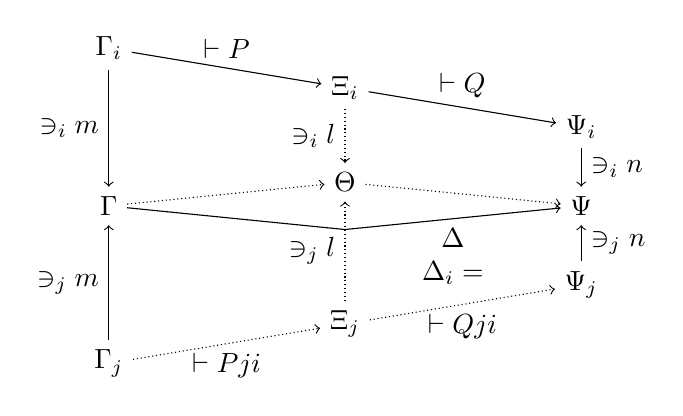
\begin{tikzpicture}
        \node (gamma-i) at (0,4)   {$\Gamma_i$};
        \node (gamma-m) at (0,2)   {$\Gamma$};
        \node (gamma-j) at (0,0)   {$\Gamma_j$};
        \node (xi-i)    at (3,3.5) {$\Xi_i$};
        \node (theta)   at (3,2.3) {$\Theta$};
        \node (delta-m) at (3,1.7) {};
        \node (xi-j)    at (3,0.5) {$\Xi_j$};
        \node (psi-i)   at (6,3)   {$\Psi_i$};
        \node (psi-m)   at (6,2)   {$\Psi$};
        \node (psi-j)   at (6,1)   {$\Psi_j$};

        \draw[-]  (gamma-m) -- (delta-m.center);
        \draw[->] (delta-m.center) -- node[align=center,below] {$\Delta$\\$\Delta_i = \lz$}(psi-m);

        \draw[->,densely dotted] (gamma-m) -- (theta);
        \draw[->,densely dotted] (theta) -- (psi-m);

        \draw[->] (gamma-i) -- node[left] {$\ni_i m$} (gamma-m);
        \draw[->] (gamma-j) -- node[left] {$\ni_j m$} (gamma-m);
        \draw[->] (psi-i) -- node[right] {$\ni_i n$} (psi-m);
        \draw[->] (psi-j) -- node[right] {$\ni_j n$} (psi-m);

        \draw[->] (gamma-i) -- node[above] {$\vdash P$} (xi-i);
        \draw[->] (xi-i) -- node[above] {$\vdash Q$} (psi-i);
        \draw[->,densely dotted] (gamma-j) -- node[below] {$\vdash \subst{P}{j}{i}$} (xi-j);
        \draw[->,densely dotted] (xi-j) -- node[below] {$\vdash \subst{Q}{j}{i}$} (psi-j);
        \draw[->,densely dotted] (xi-i) -- node[left] {$\ni_i l$} (theta);
        \draw[->,densely dotted] (xi-j) -- node[left] {$\ni_j l$} (theta);
      \end{tikzpicture}

      Diagrammatic representation of the $\comp{}{}$ case for substitution.
      Continuous lines represent known facts, dotted lines proof obligations.

  \end{itemize}  
\end{proof}

\begin{nitheorem}[Substitution]
  \label{thm:substitution}
  Let process $P$ be well typed in $\types{\gamma \comma t}{\Gamma \comma m}{P}{\Psi \comma \lz}$.
  Let $\contains{\gamma}{\Psi}{j}{t}{m}{\Xi}$.
  Then, we can substitute the variable references to $\constr{0}$ in $P$ with $\suc j$ so that the result is well typed in $\types{\gamma \comma t}{\Gamma \comma m}{\subst{P}{\suc j}{\constr{0}}}{\Xi \comma m}$.
\end{nitheorem}
\begin{proof}
  For $\contains{\gamma}{\Gamma}{j}{t}{m}{\Theta}$ and $\types{\gamma \comma t}{\Theta \comma m}{P}{\Xi \comma \lz}$ for some $\Theta$, we use framing to derive them.
  Then, we use these to apply \autoref{thm:substitution-generalization}.
\end{proof}

\paragraph*{Subject Reduction}
Finally we are ready to present our main result, stating  that if $P$ is well typed and it reduces to $Q$, then $Q$ is well typed.
The relation between the typing contexts used to type $P$ and $Q$ will be explained in \autoref{thm:subject-reduction1}.
In the \picalc{} we distinguish between a reduction $P \reduce{\constr{internal}} Q$ on a channel internal to $P$, and a reduction $P \reduce{\constr{external} \; i} Q$ on a channel $i$ external to $P$ (refer to \autoref{semantics}).
We first introduce an auxiliary lemma:

\begin{nilemma}
  \label{lm:comm-capable}
  Every input usage context $\Gamma$ of a well-typed process $\types{\gamma}{\Gamma}{P}{\Delta}$ that reduces by communicating on a channel external (that is, $P \reduce{\constr{external} \; i} Q$ for some $Q$) has a multiplicity of at least $\lio$ at index $i$.
\end{nilemma}

\begin{proof}
  By induction on the reduction derivation $P \reduce{\constr{external \; i}}Q$.
\end{proof}

\begin{nitheorem}[Subject reduction]
  \label{thm:subject-reduction1}
  Let $P$ be well typed in $\types{\gamma}{\Gamma}{P}{\Xi}$ and reduce such that $P \reduce{c} Q$.
  \begin{itemize}
    \item If $c$ is $\constr{internal}$, then $\types{\gamma}{\Gamma}{Q}{\Xi}$.
    \item If $c$ is $\constr{external} \; i$ and $\containsusage{\Gamma}{i}{\lio}{\Delta}$, then $\types{\gamma}{\Delta}{Q}{\Xi}$.
  \end{itemize}
\end{nitheorem}

\begin{proof}
  By induction on $P \reduce{c} Q$. For the full details refer to our mechanisation in Agda.  
  \begin{itemize}
    \item
    Case $\constr{comm}$: we apply framing (\autoref{thm:framing}) (to rearrange the assumptions), substitution (\autoref{thm:substitution}) and strengthening (\autoref{thm:strengthening}).
  
    \item
    Case $\constr{par}$: by induction on the process that is being reduced.

    \item
    Case $\constr{res}$: case split on channel $c$:
    if $\constr{internal}$ proceed inductively;
    if $\constr{external}\; \constr{0}$ (i.e. the channel introduced by scope restriction) use \autoref{lm:comm-capable} to subtract $\lio$ from the channel's usage annotation and proceed inductively;
    if $\constr{external}\; (\suc i)$ proceed inductively.

    \item
    Case $\constr{struct}$: we apply subject congruence (\autoref{thm:subject-congruence1}) and proceed inductively. \qed
  \end{itemize}
\end{proof}
